\subsection{External Validation on Three Further Hospitals (RQ3)}
All earlier results are internal to Cleveland. Table~\ref{tab:sites} shows that the three other UCI sites differ markedly from it. CAD prevalence ranges from 36\% (Hungary) to 94\% (Switzerland), and the two strongest Cleveland predictors are mostly unavailable: \texttt{ca} is missing for 96--99\% and \texttt{thal} for 42--90\% of patients. Models trained on all 303 Cleveland patients and applied unchanged (Table~\ref{tab:e7}, Fig.~\ref{fig:a6}) reach AUC \extHunFu{} in Hungary, \extSwiFu{} in Switzerland and \extVaFu{} at VA Long Beach (clinical-only: \extHunCl{}, \extSwiCl{}, \extVaCl{}). Fused and clinical-only models do not differ at any site (fused$-$clinical $\Delta$AUC with bootstrap CI: \extDeltaList{}).

A second edge case emerges here. When \texttt{ca} and \texttt{thal} are missing, median imputation fills them with Cleveland's medians (0 vessels, normal thallium), the values most typical of \emph{healthy} patients. Sensitivity therefore collapses at the external sites (Table~\ref{tab:e7}). Training without \texttt{ca}, \texttt{thal} and \texttt{slope} restores sensitivity to 0.77--0.85 and improves calibration (lower Brier) at the cost of specificity, and at VA it also improves AUC. A model should therefore be trained on the features that will actually be available at deployment rather than relying on imputation of its most important inputs. Cholesterol is recorded as 0~mg/dL for all 123 Swiss and 49 VA patients. Treating these values as missing rather than literally changes external AUC by at most 0.004, because cholesterol carries little weight in the model (\texttt{E7\_chol\_zero\_edge\_case.csv} in the repository).

\begin{table}[!t]
\centering
\scriptsize
\caption{Characteristics of the four UCI heart-disease sites (chol = 0 treated as missing).}
\label{tab:sites}
\setlength{\tabcolsep}{3pt}
\begin{adjustbox}{max width=\linewidth}
\begin{tabular}{lcccccc}
\toprule
Site & n & Prev. & ca miss. & thal miss. & slope miss. & chol miss. \\
\midrule
Cleveland & 303 & 45.9\% & 1\% & 1\% & 0\% & 0\% \\
Hungary & 294 & 36.1\% & 99\% & 90\% & 65\% & 8\% \\
Switzerland & 123 & 93.5\% & 96\% & 42\% & 14\% & 100\% \\
VA Long Beach & 200 & 74.5\% & 99\% & 83\% & 51\% & 28\% \\
\bottomrule
\end{tabular}
\end{adjustbox}
\end{table}

\begin{table*}[!t]
\centering
\scriptsize
\caption{External validation: trained on all 303 Cleveland patients, tested unchanged on three other hospitals.}
\label{tab:e7}
\setlength{\tabcolsep}{3pt}
\begin{adjustbox}{max width=\linewidth}
\begin{tabular}{llcccc}
\toprule
Site & Model (trained on Cleveland) & AUC [95\% CI] & Sens. & Spec. & Brier \\
\midrule
Hungary & Clinical only & 0.886 [0.844, 0.927] & 0.557 & 0.963 & 0.143 \\
Hungary & Clinical, without ca/thal/slope & 0.885 [0.844, 0.925] & 0.774 & 0.830 & 0.135 \\
Hungary & Fused (full system) & 0.889 [0.847, 0.931] & 0.670 & 0.931 & 0.133 \\
Hungary & Fused, without ca/thal/slope & 0.883 [0.841, 0.925] & 0.774 & 0.846 & 0.136 \\
Switzerland & Clinical only & 0.785 [0.596, 0.946] & 0.548 & 0.875 & 0.262 \\
Switzerland & Clinical, without ca/thal/slope & 0.792 [0.615, 0.951] & 0.817 & 0.625 & 0.150 \\
Switzerland & Fused (full system) & 0.772 [0.552, 0.959] & 0.574 & 0.750 & 0.250 \\
Switzerland & Fused, without ca/thal/slope & 0.771 [0.560, 0.941] & 0.800 & 0.625 & 0.154 \\
VA Long Beach & Clinical only & 0.721 [0.635, 0.803] & 0.463 & 0.784 & 0.261 \\
VA Long Beach & Clinical, without ca/thal/slope & 0.751 [0.672, 0.828] & 0.846 & 0.451 & 0.168 \\
VA Long Beach & Fused (full system) & 0.709 [0.622, 0.790] & 0.510 & 0.784 & 0.255 \\
VA Long Beach & Fused, without ca/thal/slope & 0.754 [0.674, 0.826] & 0.839 & 0.490 & 0.176 \\
\bottomrule
\end{tabular}
\end{adjustbox}
\end{table*}


\begin{figure}[!t]
\centering
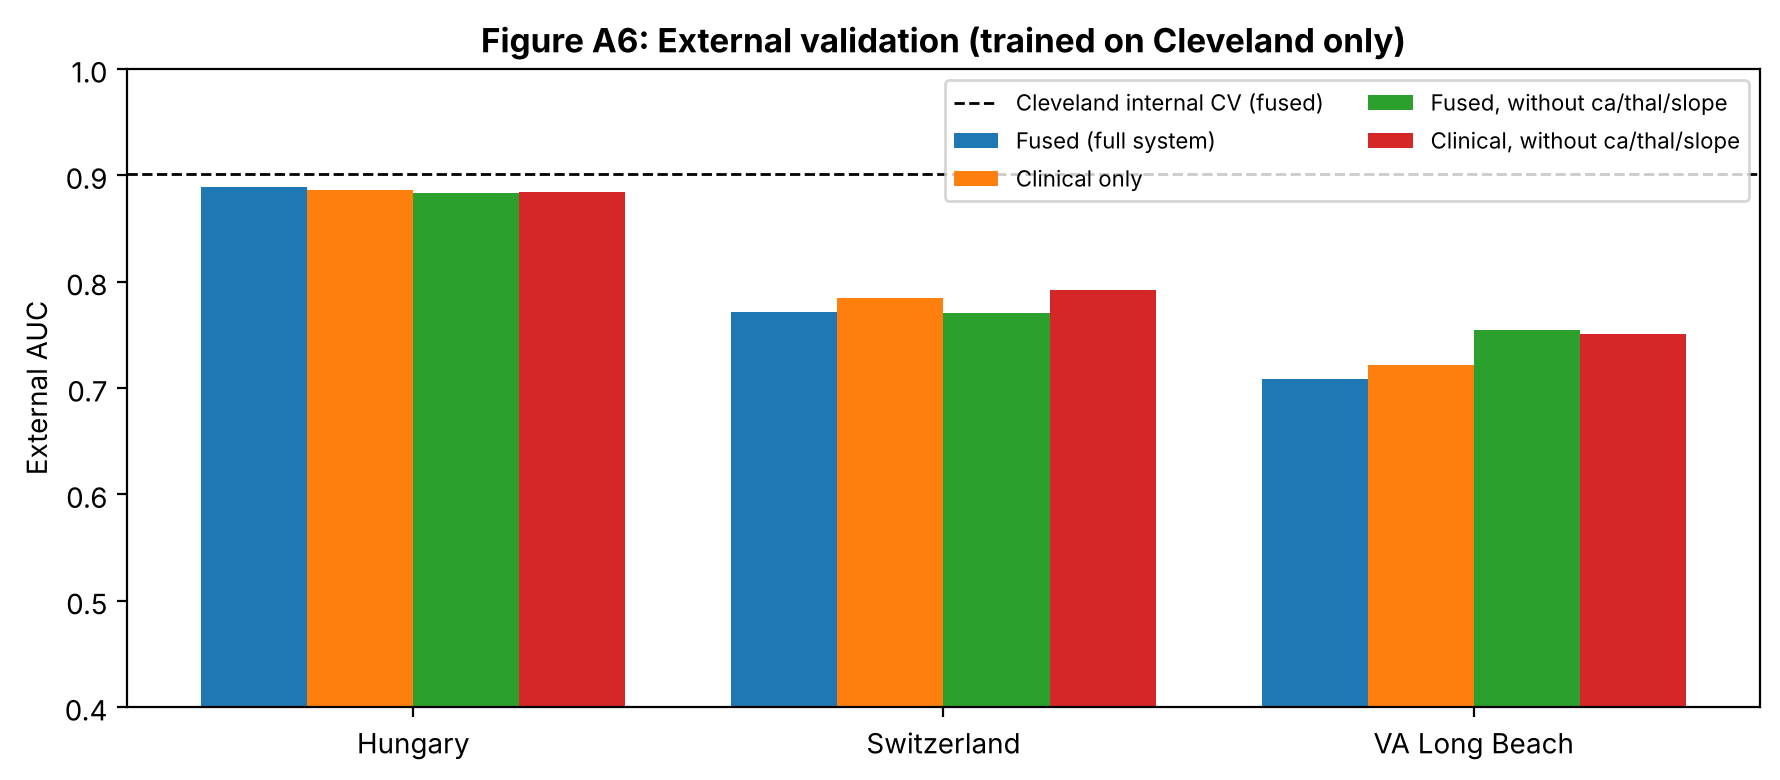
\includegraphics[width=\linewidth]{figA6_external.png}
\caption{External AUC of models trained on Cleveland only (dashed: Cleveland internal CV).}
\label{fig:a6}
\end{figure}

\subsection{SHAP Stability (RQ4)}
Attribution stability across 50 folds and 10 seeds, and agreement with permutation importance, are reported with the interpretation results in Section~VII (Tables~\ref{tab:e8} and~\ref{tab:shaptop}).

\subsection{Cross-Attention in the Dual-Branch Network}
Table~\ref{tab:e9} compares six networks trained with identical preprocessing, SMOTE and training budget. The numerical check confirms the derivation of Section~IV-C: with sequence length 1 every attention weight equals 1.000000, and replacing the ECG query with random values leaves the output unchanged. Consistent with this, the v4 architecture (AUC \xattnAUC{}) performs like its linear equivalent (\linearAUC{}) and like plain concatenation (\concatAUC{}; $\Delta$ \dConcat{}). A token-level variant, in which each ECG-proxy feature attends over the 13 clinical features so that attention can actually weight them, reaches \tokensAUC{} ($\Delta$ \dTokens{}). The token-level variant only reaches the level of the clinical-only MLP (\mlpClinAUC{}); no network exceeds it, and all remain below the soft-voting ensemble (\fullAUC{}). Adding the proxy block to an MLP actually lowers AUC (single MLP on all 36 features), as expected when 303 patients are spread over more inputs. We therefore remove cross-attention from the proposed system and report the dual-branch network only as an ablation.

\begin{table*}[!t]
\centering
\scriptsize
\caption{Dual-branch networks with and without cross-attention (identical preprocessing, SMOTE and training budget).}
\label{tab:e9}
\setlength{\tabcolsep}{3pt}
\begin{adjustbox}{max width=\linewidth}
\begin{tabular}{lcccc}
\toprule
Model (3$\times$10-fold CV) & AUC [95\% CI] & Acc. & Sens. & $\Delta$AUC vs L=1 attention \\
\midrule
Full system (clinical + ECG-proxy, SMOTE, soft voting) & 0.901 [0.859, 0.944] & 0.824 & 0.780 & +0.015 [-0.018, +0.047] \\
$-$ ECG-proxy block (clinical only) & 0.907 [0.865, 0.950] & 0.827 & 0.787 & +0.021 [-0.013, +0.054] \\
DL: clinical-only MLP (Section 14) & 0.892 [0.848, 0.936] & 0.821 & 0.787 & +0.006 [-0.023, +0.035] \\
DL: single MLP on all 36 features & 0.866 [0.826, 0.906] & 0.793 & 0.763 & -0.021 [-0.052, +0.010] \\
DL: dual branch + concatenation & 0.878 [0.828, 0.927] & 0.813 & 0.765 & -0.009 [-0.030, +0.012] \\
DL: dual branch + cross-attention (L=1, paper) & 0.887 [0.840, 0.933] & 0.812 & 0.791 & -- \\
DL: dual branch + linear layer ($\equiv$ L=1 attention) & 0.885 [0.843, 0.927] & 0.814 & 0.767 & -0.002 [-0.023, +0.019] \\
DL: dual branch + token-level cross-attention & 0.893 [0.852, 0.934] & 0.815 & 0.813 & +0.006 [-0.023, +0.036] \\
\bottomrule
\end{tabular}
\end{adjustbox}
\end{table*}


\subsection{PTB-XL ECG Branch}
The parallel ECG benchmark (D2; PTB-XL normal versus abnormal) was ablated in the same way (Table~\ref{tab:e10}). Lead~II with Efficient tsfresh features reaches AUC \ecgRefAUC{}. The choice of lead matters: V5 performs as well as Lead~II (\ecgVFiveAUC{}), while Lead~I (\ecgLeadIAUC{}) and V1 (\ecgVOneAUC{}) are weaker. The rich feature set is essential: the 10 Minimal statistics of Lead~II reach only \ecgMinIIAUC{} (significant drop), and 10 Minimal statistics from each of the 12 leads reach \ecgTwelveMinAUC{}. Adding the 12-lead statistics to the Lead-II descriptors gives \ecgTwelvePlusAUC{}, a small, non-significant gain, so with handcrafted statistics and $N=303$ most of the accessible information is already in one well-chosen lead. Fitting VarianceThreshold and scaling on all records, as in v4, has no measurable effect, and neither SMOTE nor the random forest of v4 improves on the reference. Increasing the training set to 1{,}212 records does not raise AUC appreciably (Table~\ref{tab:e10size}; \ecgSizeList{}), although accuracy and the precision of the estimate improve. Substantial gains from raw ECGs are known to require learned representations and far larger datasets~\cite{ribeiro2020}. Signal quality matters: records with PTB-XL noise or electrode annotations ($n=\ecgNoisyN{}$) are classified with AUC \ecgNoisyAUC{} versus \ecgCleanAUC{} for clean records.

\begin{table*}[!t]
\centering
\scriptsize
\caption{PTB-XL ECG-branch (D2) ablation, 303 records, 5$\times$10-fold CV.}
\label{tab:e10}
\setlength{\tabcolsep}{3pt}
\begin{adjustbox}{max width=\linewidth}
\begin{tabular}{lcccc}
\toprule
ECG-branch variant (PTB-XL labels) & AUC [95\% CI] & Acc. & $\Delta$AUC [95\% CI] & $p_{\mathrm{Holm}}$ \\
\midrule
Lead II, Efficient tsfresh, soft voting (reference) & 0.819 [0.766, 0.871] & 0.725 & -- & -- \\
VarianceThreshold + scaling fitted on all records & 0.820 [0.766, 0.874] & 0.727 & +0.001 [-0.007, +0.009] & 1.000 \\
Random Forest only (Section 13 best) & 0.786 [0.732, 0.839] & 0.695 & -0.033 [-0.073, +0.007] & 0.656 \\
No SMOTE & 0.807 [0.752, 0.862] & 0.717 & -0.012 [-0.040, +0.017] & 1.000 \\
Minimal tsfresh (10 features), Lead II & 0.666 [0.593, 0.739] & 0.589 & -0.153 [-0.234, -0.072] & 0.004 \\
Lead I, Efficient & 0.724 [0.659, 0.789] & 0.656 & -0.095 [-0.176, -0.014] & 0.182 \\
Lead V1, Efficient & 0.752 [0.695, 0.810] & 0.684 & -0.067 [-0.145, +0.012] & 0.656 \\
Lead V5, Efficient & 0.819 [0.762, 0.876] & 0.743 & -0.000 [-0.062, +0.061] & 1.000 \\
12-lead Minimal tsfresh (120 features) & 0.768 [0.714, 0.823] & 0.700 & -0.051 [-0.118, +0.016] & 0.680 \\
12-lead Minimal + Lead II Efficient & 0.823 [0.772, 0.874] & 0.740 & +0.004 [-0.024, +0.032] & 1.000 \\
\bottomrule
\end{tabular}
\end{adjustbox}
\end{table*}

\begin{table}[!t]
\centering
\scriptsize
\caption{PTB-XL Lead-II branch: effect of the number of training records (3$\times$10-fold CV).}
\label{tab:e10size}
\setlength{\tabcolsep}{3pt}
\begin{adjustbox}{max width=\linewidth}
\begin{tabular}{cccc}
\toprule
Records & Patients & AUC [95\% CI] & Accuracy [95\% CI] \\
\midrule
303 & 302 & 0.823 [0.766, 0.880] & 0.721 [0.665, 0.778] \\
606 & 605 & 0.800 [0.760, 0.841] & 0.727 [0.686, 0.768] \\
1212 & 1200 & 0.825 [0.801, 0.848] & 0.757 [0.730, 0.784] \\
\bottomrule
\end{tabular}
\end{adjustbox}
\end{table}


\begin{figure}[!t]
\centering
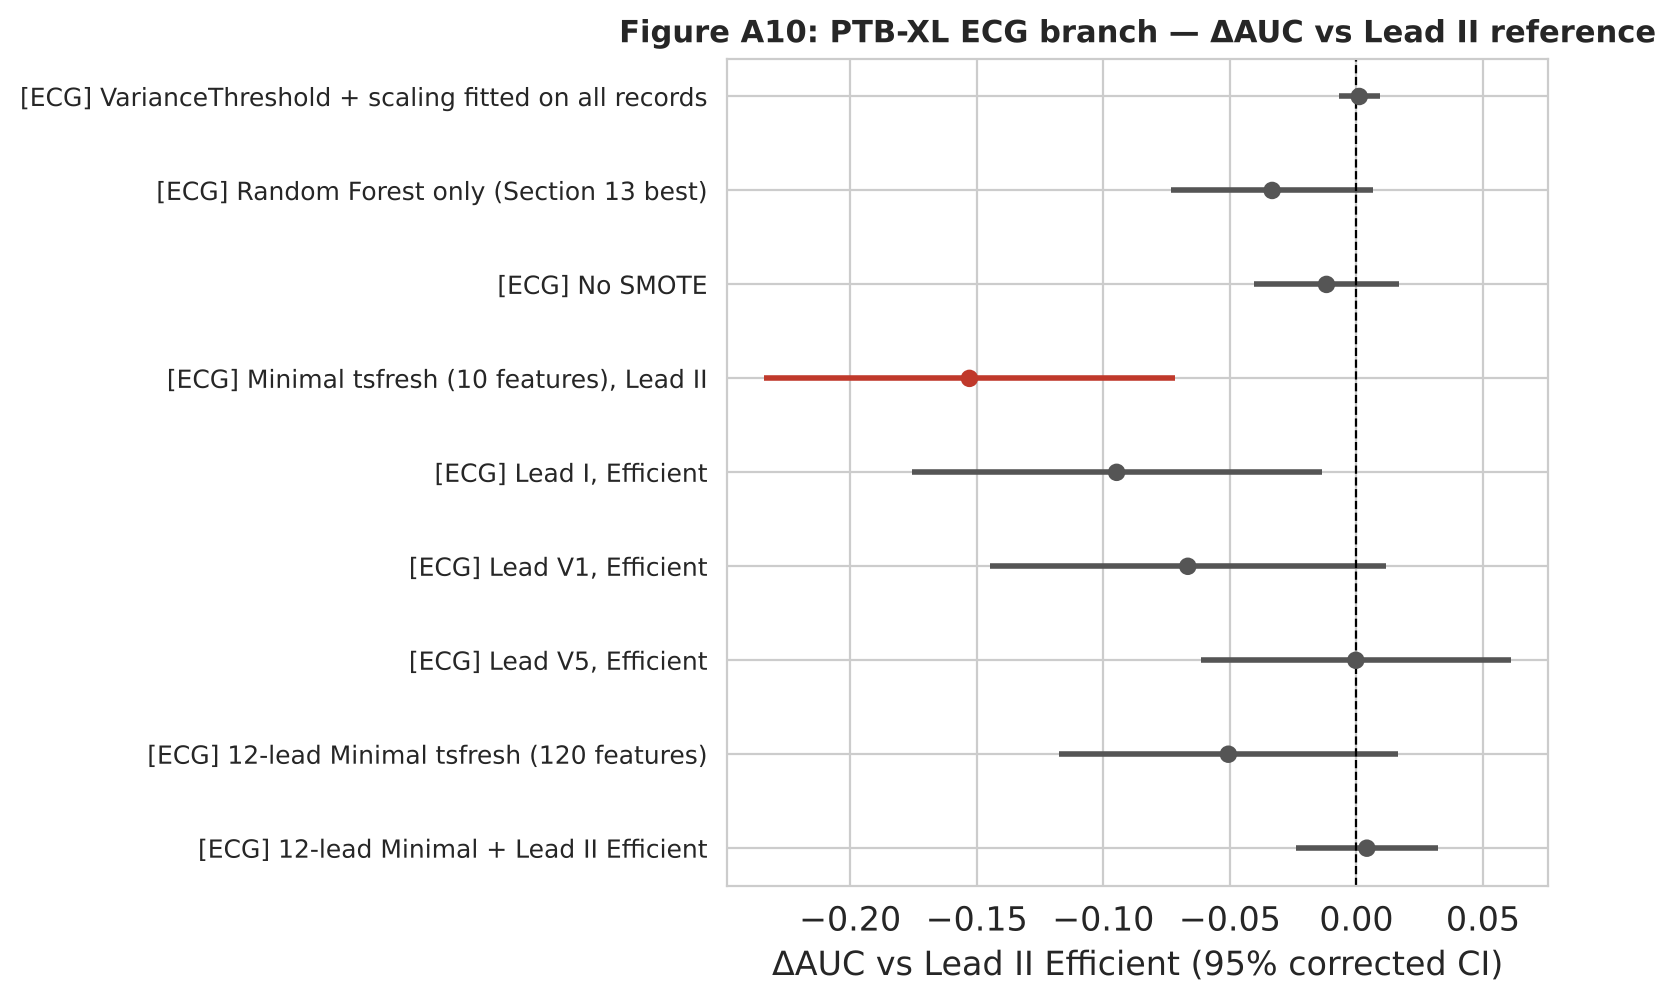
\includegraphics[width=\linewidth]{figA10_ptbxl_branch.png}
\caption{PTB-XL ECG-branch ablation: $\Delta$AUC versus Lead~II with Efficient tsfresh features.}
\label{fig:a10}
\end{figure}

\subsection{Summary: Which Claims Survive?}
Table~\ref{tab:verdict} re-tests each quantitative claim of the v4 manuscript.

\begin{table*}[!t]
\centering
\scriptsize
\caption{Claims of the v4 manuscript re-tested under the controlled protocol. A claim is supported only if the 95\% CI of the paired difference excludes zero in the claimed direction.}
\label{tab:verdict}
\setlength{\tabcolsep}{3pt}
\begin{adjustbox}{max width=\linewidth}
\begin{tabular}{p{4.6cm}p{2.6cm}p{5.6cm}p{3.6cm}}
\toprule
Claim in the v4 manuscript & v4 value & Controlled estimate [95\% CI] & Verdict \\
\midrule
ECG-proxy fusion improves accuracy over clinical-only & +7.04 pp & -0.262 pp [-2.683, +2.158] & Not supported (CI includes 0) \\
ECG-proxy fusion improves AUC over clinical-only & +0.87 pp (0.9535 vs 0.9459) & -0.004 [-0.017, +0.009] & Not supported (CI includes 0) \\
Removing the ECG-proxy layer lowers AUC & $\approx$ $-$0.06 & +0.004 [-0.009, +0.017] & Not supported (CI includes 0) \\
Removing SMOTE causes the largest drop & $\approx$ $-$3.3\% accuracy & +1.058 pp [-0.584, +2.700] & Not supported (CI includes 0) \\
Removing SMOTE lowers AUC & "noticeable drop" & -0.002 [-0.009, +0.006] & Not supported (CI includes 0) \\
Ensemble beats a single (XGBoost) classifier & AUC $-$0.014 without ensemble & -0.007 [-0.020, +0.006] & Not supported (CI includes 0) \\
Feature engineering contributes & AUC $-$0.005 without it & -0.003 [-0.023, +0.018] & Not supported (CI includes 0) \\
ECG-proxy block beats an equal-size non-ECG block & (implied) & -0.002 [-0.020, +0.016] & Not supported (CI includes 0) \\
Cross-attention improves the dual-branch network & (implied by MCF-BiModNet) & +0.009 [-0.012, +0.030] & Not supported (CI includes 0) \\
SHAP ranking is a stable basis for clinical interpretation & thal, ca, cp, oldpeak dominate & fold-to-fold Spearman $\rho$ = 0.90; top-5 Jaccard = 0.74 & Partly supported (top features stable, tail unstable) \\
Performance generalises beyond Cleveland & (not tested) & Hungary AUC=0.889, Switzerland AUC=0.772, VA Long Beach AUC=0.709 & Lower AUC at all external sites; fused $\approx$ clinical \\
Hold-out accuracy 88.52\% is representative & 0.8852 (seed 42) & 0.833 over 200 splits (seed 42 = 95th pct) & Optimistic single split \\
\bottomrule
\end{tabular}
\end{adjustbox}
\end{table*}


